The key contribution of this work is to build an environment for a single family household, consisting of a rooftop solar array for energy generation, an energy storage system, a thermostatically controlled load and flexible demand response. The enviroment is built on a mixture of simulated and real data and dynamic components. It is used to optimize the CO2eq emissions of the household. The environment is built on the Gymansium framework \cite{Towers.2023} and is available on GitHub\footnote{https://github.com/TimWalter/smart-energy-controller}
\par
The training environment was chosen to be episodic to accomodate the environment framework\cite{Towers.2023} and algorithm framework\cite{AntoninRaffin.2021}. The episodes are organized into weeks, with either minutely or hourly resolution, to capture the daily and weekly patterns of the household. The timeframe chosen, was 07.01.2007 - 28.12.2008, although some episodes had to be left out due to missing data. Overall there were more than 100 episodes, of which 95 were used for training, 4 for testing and the rest for training. The power was standarized to kilowatts, while the energy was simply kWmin or kWh depending on the resolution. As the agents is operating on equidistant timesteps anyway, there is no real difference between energy and power, as the power is always assumed to be constant over the timestep. The location of the house was in France near Paris.


\subsection{Static Components}\label{ssec:static_components}
The static components are the parts of the environment that are not reactive to the agent's actions. These are auxillary information, the generation of the rooftop solar array, the household energy demand and the external electricity supply. The data was either given in hourly or minutely resolution, and was adapted to the missing resolution using linear interpolation or averaging.

\subsubsection{Auxillary Information}\label{sssec:auxillary_information}
As auxillary information, weather and time data was given, which was sourced from the Photovoltaic Geographical Information System (PVGIS) \cite{ThomasHuld.2012}. They had no direct influence on the reward and only provided means for the agent to predict the carbon intensity of the electricity mix. The only exception was the outdoor temperature, which influenced the thermostatically controlled load. The actual observables of this component are given in table \ref{tab:observation_space}.

\subsubsection{Rooftop Solar Array (RSA)}
The generated energy was simulated using the PVLIB library \cite{F.Holmgren.2018}. The simulation used the weather data described in \ref{sssec:auxillary_information} and the solar panel specifications from the CEC database \cite{Dobos.2012}\cite{Boyson.2007}.

\subsubsection{Household Energy Demand}\label{sssec:household_energy_demand}
The household energy demand was sourced from the UCI archive \cite{GeorgesHebrail.2006}. Since the consumption was unraveled for different rooms, the kitchen, electric water heater and air conditioner were modelled as inflexible demand, while the laundry room was modelled as flexible demand.

\subsubsection{External Electricity Supply (EES)}
The direct carbon intensity of the electricity mix at any given time was sourced from electricity maps \cite{.29.12.2023} for France. However, only data from 2021 and 2022 was available, so the carbon intensity might be biased, since the electricity mix might have drifted over the years. However, the daily, weekly and yearly frequencies should still be captured, although potentially drifted. The unit of carbon intensity is gramm of CO\textsubscript{2} equivalent emissions per kWh or kWmin.

To showcase the scenario and patterns the static components are visualized for the first 24 hours in figure \ref{fig:static_components}, excluding the auxillary information.
\begin{figure}[H]
    \centering
    \setlength{\abovecaptionskip}{0pt}
    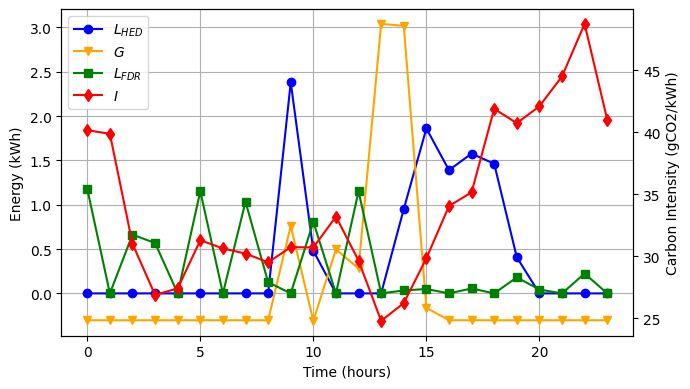
\includegraphics[width=0.45\textwidth]{figures/static_components.png}
    \caption{Static components for the first 24 hours}
    \label{fig:static_components}
\end{figure}


\subsection{Dynamic Components}\label{ssec:dynamic_components}
The dynamic components consist of an energy storage system, flexible demand response and thermostatically controlled load.

\subsubsection{Energy Storage System}
The energy storage system (ESS) is directly chargable and dischargeable from either the EES or the RSA. The charge is subject to the followng dynamics:
\begin{equation}
    B_t = \max\{0, B_{t-1} - D_s + C_t \sqrt{\nu} - \frac{D_t}{\sqrt{\nu}}\}
\end{equation}
Here, $B_t \in [0, B_{max}]$ is the charge at time $t$ and $B_{max}$ is the capacity. Furthermore, $\nu$ denotes the round trip efficiency, $D_s$ the self-discharge rate, $C_t \in [0, C_{max}]$ the charge rate with maximum $C_{max}$ and $D_t \in [0, D_{max}]$ the discharge rate with its maximum  $D_{max}$. The rates can be further constrained by the current charge and capacity, such that actually $C_t \in [0, \min\{C_{max}, \frac{B_{max} - B_t + D_s}{\sqrt{\nu}}\}]$ and $D_t \in [0, \min\{D_{max}, (B_t - D_S) \sqrt{\nu}\}]$.

\subsubsection{Flexible Demand Response}
Flexible Demand Response (FDR) denotes the shifting of load in time. This is modelled as a desired schedule of usage, as described in \ref{sssec:household_energy_demand}. A timeframe centred around the current timestep of the schedule is influenced stochatistacally by a scalar signal $a_{fdr, t} \in [-1 , 1]$. Whether a usage is executed is determined by a Bernoulli process, with probabilities $p$ calculated from the desired schedule, the signal and an exponential weighting, which is centered around the scheduled time of usage. The probabilities are given by:
\begin{equation}
    p_t = \max\{0, \min\{1, s + a_{fdr, t} * \exp(\frac{-1}{\beta}|t - t_{s}|)\}\}
\end{equation}
where $s \in \{0,1\}^{H}$ is the vector of the desired schedule with elements $s_i = \begin{cases}
    1 & \text{if } t_i \leq t \\
    0 & \text{else}
\end{cases}$ and $H$ the number of usages in the timeframe, $\beta$ is a patience parameter, and $t_{s} \in \mathbb{R}^{H}$ is the vector of desired execution times in the current timeframe. If a usage is executed its power is completely drawn in the current timestep. However, if a usage is not executed after being delayed once, it will consume a discounted amount of power in each timestep, such that if it is never exectued it will consume the same amount of power as if it was executed once. This aims to facilitate learning by preventing infinite delays or a large negative reward at the end of the episode. To do so the  power consumption of a usage after the first delay is $\frac{2p}{H-1}$, which is also discounted from the remaining power.

\subsubsection{Thermostatically Controlled Load}
The Thermostatically Controlled Load (TCL) encapsulates all devices that aim to maintain the temperature of a given heat mass. To utilize such loads as energy storage, the temperature of the heat mass is allowed to fluctuate within a given range. The TCL is modeled as a second-order system \cite{Sonderegger.1978} that has the following update procedure:
\begin{equation}
    \begin{split}
        T_t &= T_{t-1} + \frac{1}{r_a} (T_{a, t} - T_{t-1}) \\
        &+ \frac{1}{r_b} (T_{b,t} - T_{t-1}) \\
        &+ \frac{1}{r_h} L_{TCL} a_{tcl,t} + q
    \end{split}
\end{equation}
where $T$ is the indoor temperature, $r_a$ is the thermal mass of the air, $T_{a}$ is the outdoor temperature, $r_b$ is the thermal mass of the building material, and $T_{b}$ is the  building mass temperature, that evolves with
\begin{equation}
    T_{b, t} = T_{b, t-1} + \frac{1}{r_b} (T_{t-1} - T_{b, t-1})
\end{equation},
$\frac{1}{r_h}$ is the power-to-heat coefficient, $L_{TCL}$ is the nominal power, 
$a_{tcl_t} \in [-1, 1]$ is the heating signal, and $q$ is the unintentional heat drift. The heating signal is constrained by the desired temperature range, enforced through a backup controller as follows:
\begin{equation}
    a_{tcl, t} = \begin{cases}
        -1 & \text{if } T_t \geq T_{max} \\
        1 & \text{if } T_t \leq T_{min} \\
        a_{tcl, t} & \text{else} 
    \end{cases}
\end{equation}
where $T_{max}$ and $T_{min}$ define the desired temperature range. 

\subsection{Markov Decision Process}
The data in combination with the dynamic components allows the formulation of a Markov Decision Process (MDP), necessary for the RL paradigm. This requires the definition of an observation space, action space, a reward function and a transition function. The transition function is given by the replay of measurements described in \ref{ssec:static_components} and the dynamics described in \ref{ssec:dynamic_components}.

\subsubsection{Observation Space}
The observation space is a bounded subset of $\mathbb{R}^{12}$, with the observables given in \ref{tab:observation_space}. 
\begin{table}[H]
    \centering
    \begin{tabular}{lll}
    \textbf{Observable} & \textbf{Symbol} \\
    \hline
    Carbon Intensity & $I$\\
    Household Energy Demand & $L_{HED}$ \\
    Rooftop Solar Generation & $G$ \\
    ESS Charge & $B$ \\
    FDR power in current timeframe & $L_{FDR}$ \\
    Indoor temperature & $T$ \\
    Day of Year & $DoY$ \\
    Hour of Day & $HoD$ \\
    Solar Irradiation & $SI$ \\
    Solar Elevation & $SE$ \\
    Outdor temperature & $T_a$ \\
    Wind Speed & $WS$ \\
    \end{tabular}
    \caption{Observation Space}
    \label{tab:observation_space}
\end{table}

\subsubsection{Action Space}
The agent can influence the components of \ref{ssec:dynamic_components}, through the signals $a_{fdr}$, $a_{tcl}$ and $a_{ess}$. For $a_{ess}$ the charging and discharging rates are combined into a single signal, since the ESS can either be charged or discharged at any given timestep. 
All signal are normalized to $[-1, 1]$ and can be discretized into bins, if the algorithm require a discrete action space. The action space is summarized in table \ref{tab:action_space}.
\begin{table}[H]
    \centering
    \begin{tabular}{lll}
    \textbf{Action} & \textbf{Min. Meaning} & \textbf{Max. Meaning}\\
    \hline
    $a_{ess}$ & Discharge & Charge \\ 
    $a_{fdr}$ & Delay     & Expedite \\
    $a_{tcl}$ & No heating& Heating\\
    \end{tabular}
    \caption{Action Space}
    \label{tab:action_space}
\end{table}

\subsubsection{Reward Function}
The reward function is mainly given by the physical quantity of CO2eq emissions. However, to prevent unintended exploitation of the TCL, which is often optimal at constant $T_{min}$, it is augmented by a discomfort penalty. The resulting function is given by:
\begin{flalign}
    r_t &= I_t (PE - CE) - DC && \\
    \begin{split}
        EC &= L_t + \frac{1}{r_h} L_{TCL} a_{tcl,t} + C_t \\
        &+ \sum_{p \in U_e} p_r + \sum_{p \in U_d} \frac{2p}{H-1}
    \end{split} && \\
    E_p &= G_t + D_t  && \\
    DC &= \delta exp(|T_t - \frac{T_{max} + T_{min}}{2}) &&
\end{flalign}
where $PE$ is the energy produced, $CE$ is the energy produced, $U_e$ is the set of executed usages, $p_r$ is the remaining power after discounting, $U_d$ is the set of delayed usages, $DC$ is the discomfort with a penalty factor $\delta$. 
\par
Moreover, since the task is episodically formulated, there is a correction necessary at the end of the episode to account for e.g. differences in charge left. The correction of the final reward is given as:
\begin{flalign}
    reward &\mathrel{+}= I_t * B_t && \\
    reward &\mathrel{+}= I_t * (- \sum_{p \in U} p_r) && \\
    reward &\mathrel{+}= I_t * (- r_h|T_t - \frac{T_{max}+T_{min}}{2}|) && 
\end{flalign}
where $U$ is the set of left over usages. Every equation is correcting for one type of left over energy in the system.